\documentclass[10pt,letterpaper]{article}
\usepackage[latin1]{inputenc}
\usepackage{amsmath}
\usepackage{amsfonts}
\usepackage{amssymb}
\usepackage{graphicx}
\usepackage{parskip}
\usepackage{todonotes}
\usepackage{url}


\newtheorem{example}{Example}[section]
\newtheorem{discussion}{Discussion}[section]
\newtheorem{excercise}{Excercise}[section]
\newtheorem{algorithm}{Algorithm}[section]

\newcommand{\set}[1]{\{#1\}}

\title{Draft Technical Notes on BayesDB}
\begin{document}

\maketitle
\section{Overview: Generative Population Models and the BayesDB Minimal Modeling Language}
\label{sec:overview}

BQL programs are executed against a set of ambient data \textit{generative
population models} (GPMs), with one GPM per table in the database. These
generative population models are provided by BayesDB based on modeling schemas
and inference programs written in the BayesDB Minimal Modeling Language (MML).
Each GPM induces a random table $\mathbf{X}$ with a finite  number of columns
and an infinite number of rows. Some of the rows are observed and represent the
actual dataset stored in BayesDB. Each cell $\mathbf{X_{ij}}$ in the table
represents a random variable, and may have one or more realizations
$x_{ij}^{(t)}$.

\todo{Note sure how to formalize this in a tabular form.}
A GPM $\mathcal{G}$ can simulate and evaluate the probability of an arbitrary
collection of cells in the random table, for either observed or hypothetical
rows.

In its simplest form a GPM $\mathcal{G}$ is a fixed object that fully
characterizes a data generating process, and observing generated members has no
bearing on the actual structure.

\begin{example} \label{ex:normal_gpm} A Pretty Normal Generative Population Model

Consider a GPM $\mathcal{G}$ which simulates $D$-dimensional members of a
statistical population according to a mixture of two normal distributions such
that $p(x)= w_1\mathcal{N}(x;\mu_1,\Sigma_1) +
w_2\mathcal{N}(x;\mu_2,\Sigma_2)$. The \textit{structure} of the GPM can be
thought of as:
\begin{itemize}

\item The generative population model class $\mathcal{M}$ from which this GPM
 $\mathcal{G}$ is derived. Here $\mathcal{M} = \set{M_i^\theta \textit{: mixture
 of } i \textit{ normals with parameters } \theta}$.

\item  The member of the class corresponding to $\mathcal{G}$. In this case,
$\mathcal{G}=M_2^{\theta^*}$ is indexed by $i^*=2$ (the number of components)
and parameters $\theta^*$ = $\set{w_1,w_2,\mu_1,\mu_2,\Sigma_1,\Sigma_2}$.
\end{itemize}

A population with $N$ members $\{X^{(i)} := (X_1^{(i)},\dots,X_D^{(i)})
\}_{i=1}^N$ generated by $\mathcal{G}$ is represented in BayesDB as a data table
$\mathbf{X}$ with $D$ columns and $N$ rows.
\end{example}

The GPM in Example \ref{ex:normal_gpm} is not particularly interesting. The
detailed statistical characteristics of the GPM are fixed, but such information
is rarely known a-priori
\footnote{One plausible
scenario in which a `fixed' GPM of this form can arise is if a user learns about
the structure externally from the MML. Once the GPM is ported to BayesDB, the
user decides no further inference or learning should occur.}.

In typical applications we are interesting in \textit{learning the structure of
the GPM from data}. In fully generality, this might be learning the specific
parameters $\theta$ given a fixed generative process $M_i$, or learning the
generative process $M_i$ from some fixed model class $\mathcal{M}$, or even
learning the model class itself $\mathcal{M}$ from a set of competing model
classes $\set{\mathcal{M}_k}$. The Minimal Modeling Language provides a
framework for jointly learning the structure of a collection of GPM
$\set{\mathcal{G}_i}$ that interact with another to produce a statistical
population.

A GPM $\mathcal{G}$ which can be learned from data is referred to as learnable
generative population model. A learnable GPM $\mathcal{G}$ is probabilistic
model defined over a space of GPMs. We will see in Section
\ref{sec:learnable_gpm} that a learnable GPM is a GPM in its own right and can
answer the same questions about the statistical population $\mathbf{X}$. The MML
includes a
\textit{default learnable generative population model} which defines a
distribution over a collection of
\textit{GPMs from a default class} using a hierarchal, semi-parametric Bayesian
model derived from CrossCat.

\begin{example} \label{ex:crosscat} What Exactly Is CrossCat?

A cross-categorization of a data table $\mathbf{X}$ with $D$ columns and $N$ is
a partition of the columns $(X_1,\dots,X_D)$ into blocks called \textit{views}.
In each view, we have a partition of the rows $(X_1^{i},\dots,X_D^{i})_{i=1}^N$
into blocks called \textit{categories}.

\begin{figure}[ht]
    \centering
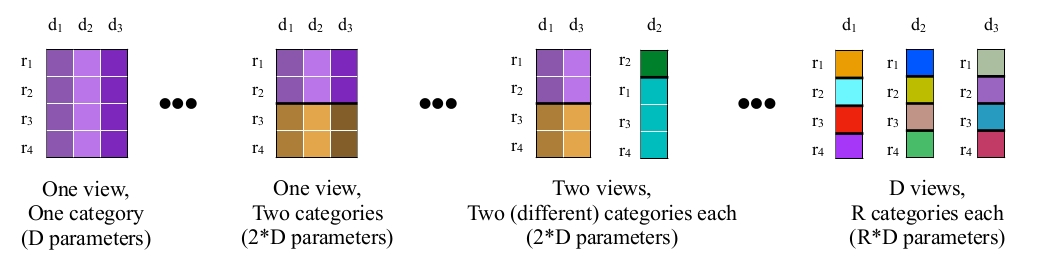
\includegraphics[width=0.8\textwidth]{cc.jpeg}
\caption{Some possible cross-categorizations of a table with 3 rows and 4
columns. The CrossCat model is very complex and contains several parameters such
as the row partition, the column partition, and component parameters (which are
shared by cells of the same color). Any two cells with a different color are
marginally independent conditioned on the entire latent structure.}
\label{fig:cc}
\end{figure}
The collection of all possible column/row partitions $j$ and associated
component parameters $\theta$ of $\mathbf{X}$ defines a GPM class:

$\mathcal{M}_\textbf{X} = \set{CC_j^{\theta} \text{ : cross-cat of } \mathbf{X}
\text{ with partition } j \text{ and component model params } \theta}$.

A member $\mathcal{G}$ of the CrossCat GPM class is a particular cross-
categorization and component parameters $CC_j^{\theta^*}$ from the model class.
Since we do not know $j$ or $\theta^*$, we instead place distribution over all
GPMS with this common structure. The object which carries this distribution over
$\mathcal{M}_\textbf{X}$ is a learnable generative population model, whose
population members are GPMs that generate the $\mathbf{X}$!

Unlike Example \ref{ex:normal_gpm}, the generation process is inherently tied to
the statistical population it has produced $\mathbf{X}$. Observing more
generated members $\mathbf{X} \to
\mathbf{X}'$ means the GPM class under consideration grows from
$\mathcal{M}_\textbf{X}$ to $\mathcal{M}_\textbf{X'}$ (both the number of
possible cross-categorizations $j$ and the dimensionality of the vector of
latents $\theta$ increase).

\todo[inline]{The reason I am being so pedantic about this construction is to
explicate various design choices when simulating, sampling, and running
posterior inference. In particular we are going to have to break down the latent
structure into 'global' vs 'row-related' latents to differentiate between
observed and hypothetical members.}
\end{example}

The default learnable GPM is not obliged to model all columns jointly by
positing some GPM from the CrossCat class. The MML includes modeling
instructions for describing dependence constraints, and specifying a
compositional, directed-acyclic network of arbitrary GPMs implemented by a user.
It also includes inference instructions for initializing learnable GPMs and
performing updates of the posterior distribution on GPMs.

The MML is thus a complete (but sub- Turing) probabilistic programming language
that interoperates with queries written in BQL. The set of primitive GPMs can be
extended by loading foreign GPMs written in VentureScript, and can be used to
transparently integrate models from disparate probabilistic programming
languages such as Stan and statistical computing environments such as R. Because
BQL programs only depend on the statistical data types of the columns, the
underlying modeling technologies, GPM assumptions, and inference tactics can be
changed without invalidating end-user data analysis workflows.

\section{Interface for Generative Population Models} \label{sec:generators}
A \textit{generative population model} is a probabilistic model of a data
generating process and a statistical population that it has produced. It is
informative to think of this statistical population as an infinite table
$\mathbf{X}$ with a finite number of columns $D$ (representing attributes) and
an infinite number of rows (representing members of the population). A finite
number of rows $r_i \in
\set{1,\dots,N}$ are actually observed, so $\mathbf{X}$ is stored in BayesDB as
an $N \times D$ table. Hypothetical members are indexed by drawing a row index
$r^*\sim U[0,1]$, which guarantees their uniqueness.

\begin{discussion} \label{disc:iid} Technical Aside On IID Rows

The classical statistical framework generally assumes that all members of a
population are independent and identically distributed. While a particular
generator is free to make any assumptions about its population, the IID
assumption is a strong one. The default generator (and almost any generator
being learned under the Bayesian framework) will usually assume that the rows
are not IID but exchangeably coupled. Di Finetti's theorem guarantees that there
exists a mixture of random measures $\set{\mathcal{G}_\alpha}$ (which in most
cases is indexed by the latent state of the GPM) where the population is
conditionally IID.

$$p(\mathbf{X}) = \int_\alpha{(\Pi_{i=1}^Np(\mathbf{X}_i|\mathcal{G}_\alpha))d
\mathcal{Q}(\mathcal{G}_\alpha)}$$

The Di Finetti measure $\mathcal{Q}$ is the object which defines a distribution
over the (fixed) measures (GPMs) that produce a statistical population. In this
sense, $\mathcal{Q}$ represents the learnable GPM.

\end{discussion}

Generative population models provide the primitive statistical inferences that
are used by BayesDB to implement inferential queries in BQL. To support all of
BQL, a GPM must provide the ability to \textbf{sample from} and \textbf{evaluate
the log density} of all possible marginal distributions subject to equality
constraints for arbitrary subsets of variables. The interface for
\textit{initializing} and \textit{querying} GPMs is outlined below.

\begin{enumerate}

\item \texttt{$\mathcal{G}$ = initialize( schema = $\Lambda$)}

    Initialize a GPM with the given schema, and return the resulting GPM
    $\mathcal{G}$.

    Each GPM is initialized with a \textit{schema} $\Lambda=$\path{(typed-
    outputs, typed-inputs, body)}. The \path{typed- outputs} component species
    the column indexes and statistical types of each column that the GPM will be
    responsible for generating. The \path {typed-inputs} component specifies the
    indexes and statistical types of columns that the data generator can read
    from. The \path{body} is an opaque binary that contains any generator
    specific configuration information, such as a probabilistic program.

\item \texttt{$\set{\vec{s}_i}_{i=1}^N$ = 
    simulate($\mathcal{G}$, targets = $\set{(r_i^t,c_i^t)}_{i=1}^{|T|}$, givens
    = $\set{(r_i^g, c_i^g, x_{(r_i^g, c_i^g)})}_{i=1}^{|G|}$, samples = $N$)}

    Generate $N$ samples from the specified conditional distribution.
    $$
    \set{\vec{s}_i}_{i=1}^N \sim p( \set{ \mathbf{X}_{(r_i^t,c_i^t)} } |
    \set{ \mathbf{X}_{(r_i^g,c_i^g)} = x_{(r_i^g,c_i^g)} }, \mathcal{G})
    $$

    Note that each $\vec{s}_i$ is a $|T|$ dimensional vector

\item \texttt{$\log p$ =
    logpdf($\mathcal{G}$, targets = $\set{(r_i^t, c_i^t, x_{(r_i^t,
    c_i^t)})}_{i=1}^{|T|}$, givens = $\set{(r_i^g, c_i^g, x_{(r_i^g,
    c_i^g)})}_{i=1}^{|G|}$}

    Evaluate the log probability density of the specified conditional
    distribution at a target point.

    $$
    \log p = p( \set{ \mathbf{X}_{(r_i^t,c_i^t)} = x_{(r_i^t,c_i^t)} } |
    \set{ \mathbf{X}_{(r_i^g,c_i^g)} = x_{(r_i^g,c_i^g)} }, \mathcal{G})
    $$

\end{enumerate}

For a BayesDB table $\mathbf{X}$ with $D$ columns and $N$ rows, the allowed
values for the indexes are
    \subitem $c_i \in \set{1,\dots,D}$
    \subitem $r_i \in \set{1,\dots,N} \cup [0,1]$

The implications of this restriction are that the MML does not have a notion of
a hypothetical column. The row indexes in $\set{1,\dots,N}$ correspond to
observed rows, while $r_i \in [0,1]$ are hypothetical members whose uniqueness
is guaranteed by simulating from the uniform distribution on the unit interval.

While the requirement that the GPM should respond to questions about arbitrary
cells in the random table may appear overwhelmingly complex, the structure of
most GPMs induces several internal simplifications.

\section{Extended Interface for Learnable Generative Population Models}
\label{sec:learnable_gpm}

As outlined in Section \ref{sec:overview}, some GPMs can be learned from an
observed statistical population $\mathbf{X}$. Learning the GPM structure will be
based on approximate probabilistic inference in a \textit{learnable generative
population model} $\mathcal{G}$ which is a probabilistic model defined over a
space of GPMs $\set{\mathcal{G_\alpha}}$. The GPMs $\mathcal{G}_\alpha$
typically share structure (such as belonging to the same parametric class) but
this is not a formal restriction.

A key insight about a learnable GPM $\mathcal{G}$ is that it can \textit{answer
the same questions about the underlying statistical population} $\mathbf{X}$
that any one of its GPMs $\mathcal{G}_\alpha$ can. These questions are answered
achieved by an appropriate sequence of sampling, conditioning, and
marginalization operations over the space of GPMs $\mathcal{G}_\alpha$.
Moreover, a learnable GPM $\mathcal{Q}$ can itself define a distribution over a
space of learnable GPMs, up to an infinitely deep level of recursion.

Thus far, all learnable GPMs in BayesDB have been based on \textit{Markov chain}
methods. These learnable GPMs internally maintain a sample from an approximate
posterior over GPMS, and provide a Markov chain transition operator that updates
the sample stochastically. Some Markov chains are \textit{asymptotically
Bayesian} in the sense that the distribution that results from sequences of $T$
updates converges to the posterior over GPMs as $T$ tends to infinity.

The extended interface for learnable GPMs based on Markov chains is outlined
below:

\begin{enumerate}

\item \texttt{$\mathcal{G}$ = initialize(schema = $\Lambda$)}

    Initializes a learnable GPM with the given schema \texttt{$\Lambda$ =
    (typed-outputs, typed-inputs, body)}, and returns an arbitrary
    initialization $\theta_\mathcal{G}^0$ and empty tabular data store
    $\mathbf{X}_\mathcal{G}$.

    \todo[inline]{If there are columns in \texttt{typed-outputs} or \texttt
    {typed-inputs} for which no generative procedure is defined in
    \texttt{body}, then the default GPM will be used to jointly model those
    columns. This is required because the MML needs a full generative model to
    query arbitrary patterns of population members. Otherwise several important
    queries would be ill-defined (for instance, simulating an output without
    conditioning on an input).}

\item \texttt{incorporate(value = $(r_j,c_j,x_{(r_j,c_j)})$)}

    Records an observation $x_{(r_j,c_j)}$ in the cell $\mathbf{X_{r_j,c_j}}$.
    If there is no row $r_j$, a new one will be created.

    Errors result from overwriting existing cells, or inserting values
    $x_{(r_j,c_j)}$ incompatible with the meta-schema $\Lambda$ (for example
    providing a wrong data type).

\item \texttt{remove($(r_j,c_j$)}

    Removes the observation $x_{(r_i,c_j)}$ stored in cell $\mathbf{X}_{ij}$.

\item \texttt{infer(program = $\mathcal{P}$)}

    Simulate an internal Markov chain transition operator $\mathcal{T}$ based on
    the inference procedure specified in the program $\mathcal{P}$.

    This inference program is typically designed in cohesion with the
    \texttt{body} specified in the schema $\Lambda$. Each run of \texttt{infer}
    improves the quality of the posterior sample.
\end{enumerate}

Some Markov chain GPMs are \textit{asymptotically Bayesian}:

\begin{equation*}
\lim_{t\to\infty}D_{KL}(p(\theta_\mathcal{G}|\mathbf{X_\mathcal{G}}) ||
p(\mathcal{T}^t(\theta_\mathcal{G}))) = 0
\end{equation*}

A sufficiently expressive asymptotically Bayesian Markov chain GPM may also be
\textit{asymptotically consistent} in the usual sense.

\section{An Ensemble of Learnable Generative Population Models}
\label{sec:ensemble}

If BayesDB inferences were based on a single instance of a learnable GPM, the
inferences would arbitrarily suppress modeling uncertainty. The MML provides an
alternative constructor for learnable GPMs that internally manages and ensemble
of GPMs. In the language of Markov Chains, the ensemble represents a set of
independent, parallel chains.

\begin{enumerate}
\item \texttt{$\mathcal{Q}$ = initialize(schema = $\Lambda$, count = S)}

    Initializes a collection of $N$ GPMs with the schema $\Lambda$.
    $$
    \mathcal{Q} = 
    (\set{\mathcal{G}_s = (\theta_{\mathcal{G}}^{(s,0)})}_{s=1}^S,
    \mathbf{X_\mathcal{Q}})
    $$

    Note that the schema and data store are shared across all GPMs in the
    ensemble.
\end{enumerate}

The default ensemble GPM maintains a uniform distribution over all $N$ GPMs and
approximately marginalizes over the posterior on GPMs via the appropriate form
of simple Monte Carlo.

\begin{enumerate}
\item \texttt{simulate} delegates to a randomly sampled Markov chain GPM
$\mathcal{G}_k$ for each of the $N$ samples in the returned set.

    $$
    \set{\vec{s}_i} = \cup_k \texttt{simulate} (\mathcal{G}_k,\dots,\texttt{size} = 1) \text{ where }
    \mathcal{G}_k \sim U[\set{\mathcal{G}_s}]
    $$

\item \texttt{logpdf} forms a Monte Carlo estimate of the expected density using
all of the GPMs in the ensemble.

    $$
    \log p = \frac{1}{S}\sum_s\texttt{logpdf}(\mathcal{G}_s)
    $$
\end{enumerate}

Other functions in the GPM interface are defined analogously. More elaborate
methods such as likelihood weighting of posterior samples from each chain are a
possible extension.

\begin{excercise} \label{ex:normal_vs_normal} Testing the Default Generative
Population Model

    Consider a learnable GPM $\mathcal{G}_N$ which defines a distribution over
    the space of mixture of Gaussian GPMs of the form seen in Example
    \ref{ex:normal_gpm}. Rather than fix the parameters as we did earlier, now
    place a prior over the number of Gaussian components $i$ and the weights,
    means, and covariances $\theta$. Also consider the default GPM
    $\mathcal{G}_{CC}$ from Example \ref{ex:crosscat}, which has a vague prior
    over the cross-categorizations and mixture parameters.

    Suppose a population $\mathbf{X}$ is observed, and we are interested in
    comparing the two GPMs. If you know about the internals of CrossCat, it
    should be clear that the collection of GPMs that $\mathcal{G}_N$ can
    generate is a subset of the GPMs generated by $\mathcal{G}_{CC}$ (how?).

    How can you invoke the GPM interface to test the performance of the default
    metamodel? (Hint: first define a set of ``performance'' metrics and a
    synthetic dataset). Does it make sense for $\mathcal{G}_N$ to outperform
    $\mathcal{G}_{CC}$ in certain regimes? Can you think of other GPMs that are
    special members of the default GPM class (hint: Naive Bayes, \dots), and
    associated tests?
\end{excercise}

\section{Characterizing Probabilistic Dependence}

Many analysis subproblems correspond directly to invocations of the GPM
interface. For example, missing or unknown values can be inferring an set of
results via \texttt{simulate} and reducing these to a point estimate. MAP
prediction can be approximated the single result with the highest likelihood
under \texttt{logpdf}.

The GPM interface is also sufficient to implement generic mechanisms for
characterizing context-specific conditional dependence and independence. This
mechanism can be used to implement additional measures that are useful for data
analysis, such as a context-sensitive measure of similarity.

Below are a collection of queries that can be answered using semantics from the
GPM interface. Consider a GPM $\mathcal{G}$ ascribing to either the primitive or
learnable GPM interface.

\begin{enumerate}
\item $\set{I_k} = \texttt{CMI}(
    \mathcal{G},
    A = \set{(r_i^a,c_i^a)}_{i=1}^{|A|}, B = \set{(r_i^b,c_i^b)}_{i=1}^{|B|}, C
    = \set{(r_i^c,c_i^c)}_{i=1}^{|D|}, D =
    \set{(r_i^a,c_i^a,x_{(r_i^a,c_i^a)})}_{i=1}^{|D|},
    \texttt{ accuracy} = N,
    \texttt{ size} = K)$

    CMI is an abbreviation of \texttt{conditional-mutual-information}
    $(A:B|C,D=d)$ under the given GPM. Let $A$, $B$, $C$, and $D$ be subsets of
    the random variables in the infinite random table $\mathbf{X}$ induced by
    the GPM. An important special case in which \texttt{CMI} can be used to
    compute bivariate, unconditional mutual information for distinct variables
    will have $C,D = \emptyset$, $A = \set{(c_1^a,r^*)}$ and $B =
    \set{(c_1^b,r^*)}$, with $r^* \sim U[0,1]$ and $c_1^a \ne c_1^b$.

    One implementation of \texttt{CMI}, applicable to all generators, is Monte
    Carlo estimation as follows.

    \begin{algorithm} \label{alg:cmi}
    First generate a collection of $N$ samples from $(A,B,C)|D=d$, each
    corresponding to a unique member of the population.

    \begin{align*}
    r_i &\sim U[0,1] \text{ where } i \in \set{0,\dots,N-1}\\
    \set{(\hat{a}_i, \hat{b}_i, \hat{c}_i)} &\sim (A,B,C)|D=d\\
    \end{align*}
    These samples can be used to form a Monte Carlo estimate of the desired
    conditional mutual information.

    \begin{align*}
    I(A:B|C,D=d) &:=
        \int \log \frac{p_{C|D=d}(c) p_{A,B,C|D=d}(a,b,c)}
            {p_{A,C|D=d}(a,c) p_{B,C|D=d}(b,c)}dF_{A,B,C|D=d}(a,b,c)\\ & \approx
        \sum_{(a,b,c)\in\set{(\hat{a}_i,\hat{b}_i,\hat{c}_i)}}
         \frac{p_{C|D=d}(\hat{c}_i) p_{A,B,C|D=d}(\hat{a}_i,\hat{b}_i,\hat{c}_i)}
         {p_{A,C|D=d}(\hat{a}_i,\hat{c}_i) p_{B,C|D=d}(\hat{b}_i,\hat{c}_i)}
    \end{align*}

    \end{algorithm}

    The output of \texttt{CMI} is set of $K$ estimates $\set{I_k}$, where each
    estimate is created using $N$ samples. This allows us to characterize
    uncertainty over the true value by computing Monte Carlo standard errors and
    other quantities of interest.

    Note that the samples are generated by invoking
    \begin{align*}
    {\tt simulate(} \mathcal{G}, {\tt targets} =
    \set{(r^,c_i^a)}\cup\set{r^,c_i^b}\cup\set{r^,c_i^c}, {\tt givens} =
    \set{(r_i^b,c_i^b,x_{(r_i^b,c_i^b)})}, {\tt size} = 1)
    \end{align*}
    and the densities in the estimated are evaluated by invoking the
    corresponding \texttt{logpdf} command. An alternative implementation of
    Algorithm \ref{alg:cmi} would be to sample a single row index $r^* \sim
    U[0,1]$ and using $N$ samples.
\end{enumerate}

\end{document}

